\documentclass{article}
% Language setting
% Replace `english' with e.g. `spanish' to change the document language
\usepackage[english]{babel}
\usepackage{csquotes}

% Set page size and margins
% Replace `letterpaper' with `a4paper' for UK/EU standard size
\usepackage[letterpaper,top=2cm,bottom=2cm,left=3cm,right=3cm,marginparwidth=1.75cm]{geometry}
% Useful packages
\usepackage{amsmath}
\usepackage{graphicx}
\usepackage[colorlinks=true, allcolors=blue]{hyperref}

\usepackage{biblatex} %Imports biblatex package
\addbibresource{ensembles.bib}
\addbibresource{nmr.bib}
\addbibresource{nmr-eq.bib}
\addbibresource{bayesian-eq.bib}
\addbibresource{cryo-em.bib}
\addbibresource{motivation.bib}

% Custom commands
\newcommand{\refsec}[1]{Section~\ref{#1}}
\newcommand{\reffig}[1]{Figure~\ref{#1}}
\newcommand{\mat}[1]{\mathbf{#1}}


\title{Intrinsically Disordered Proteins}
\author{Maeve Andersen}

\begin{document}
\maketitle

\begin{abstract}
    The structure and dynamics of intrinsically disordered proteins (IDPs) represent an active field of research in biophysics.
    Previous methods developed to describe protein structure and dynamics assume the protein to be ordered, in that the protein has a native conformation with some conformational varDescribing IDPs quantitatively requires many more degrees of freedom than experiment alone can provide.
    Thus, novel approaches to quantifying IDPs have been developed that take advantage of both computational theory and experiment. 
 In this paper, I will review IDPs. In particular I will review their core phenomena, their dynamics via a toy model of protein transitions using the energy landscape model, how IDPs are measured using Nuclear Magnetic Resonance, and finally how IDPs are studied today using a combination of computational methods and experimental measurements.
\end{abstract}


\section{Introduction}

Intrinsically disordered proteins (IDPs) represent an active area of research in protein science.
Characterization of IDPs is important as they are involved in cellular signaling and regulation,\cite{wrightIntrinsicallyDisorderedProteins2015}
and are associated with human diseases, such as neurodegenerative disease, cardiovascular disease, amyloidoses, cancer, and diabetes.\cite{uverskyIntrinsicallyDisorderedProteins2008}
Although challenging, modern methods of characterizing IDPs can provided new insights to crutial protein function human biological mechanisms. \cite{bonomiSimultaneousDeterminationProtein2018}.

\section{Conformational Ensembles}

In order to describe the structure of proteins with a high degree of heterogenuity, conformational ensembles are used \cite{lindorff-larsenSimultaneousDeterminationProtein2005},\cite{bonomiPrinciplesProteinStructural2017},\cite{thomasenConformationalEnsemblesIntrinsically2022}. 
When determining conformational ensembles, neither experiment or computational model can be used in isolation  \cite{bonomiPrinciplesProteinStructural2017}, \cite{lindorff-larsenSimultaneousDeterminationProtein2005}, \cite{schneidman-duhovnyUncertaintyIntegrativeStructural2014}. 
The reason why experiment fails to soley determine structure is is that data collected from experiment is sparse, meaning the number of unique observations is less that the degrees of freedom  \cite{schneidman-duhovnyUncertaintyIntegrativeStructural2014}. 
Computational methods such as Monte Carlo or molecular dynamics also fall short to determine protein structure for two reasons \cite{bonomiPrinciplesProteinStructural2017}:
1) The force fields used in in even the most advanced methods are still approximations. This can lead to large errors in predicted properties of proteins.
2) Limited computational resources put an upper bound on the protein simulation time.
    This means that these methods may "run out of time" before a conformational space is fully explored.
 
The most promising method of determining protein structure is to combine data from experiment with computational methods is a promising method of protein structure determination \cite{bonomiPrinciplesProteinStructural2017} ,\cite{thomasenConformationalEnsemblesIntrinsically2022} ,\cite{lindorff-larsenSimultaneousDeterminationProtein2005}.
When doing a combined approach, usually 4 components are incorperated \cite{thomasenConformationalEnsemblesIntrinsically2022}.
1) One or more experiments whose data gives information on protein strucure.
2) A method to sample protein conformations computationally.
3) A forward model, which calculates experimental observables from the conformational ensemble.
4) A refinement method, which refines the ensemble based on experimental data.

It is important to note that the term "ensemble" is often not carefully used within the field of structural biology.
In statistical mechanics, a protein's ensemble, given some set of conditions, is a probabability distribution over all possible conformations of that protein.
In structural biology, the term is overloaded with several meanings.\cite{gaalswykEmergingRolePhysical}
There is of course a thermodynamic ensemble, which refers to the distribution of a protein's conformations under thermal equilibrium.
Additionally there are uncertainty ensembles, which are collections of conformations that are degenerate due to sparse, ambiguous, or noisy data.
Uncertainty ensembles may be further broken down depending on their source.
For example, they may come from an arbitrary algorithm, or they may come from a well defined distribution.\cite{gaalswykEmergingRolePhysical}
In the next section I will describe an explicit construction of one of these enembles, as give a sense of how conformational ensemble are used and discussed in structural biology and biophysics. 


\subsection{Structural Ensemble Representation}
\begin{figure}[t]
    \centering
    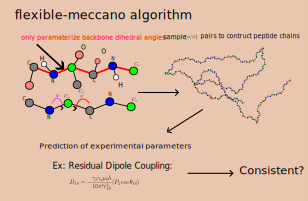
\includegraphics[width=0.75\textwidth]{flexible-meccano}
    \caption{
        Flexible-meccano, an algorithm where dihedral angles are randomly sampled to contruct a set of conformations. 
        The resulting set of conformations is considered the structural ensemble.
        Experimental parameters are then calculated for each conformation in the ensemble. 
        The calculated results are averaged and compared to the observed experiment.
        If the aggrement is good, then the set of conformations may be close to the "true" ensemble \cite{ozenneFlexiblemeccanoToolGeneration2012}.
        \label{fig:flexible-meccano}
    }
\end{figure}
A structural ensemble can be represented as a set of structures ${s_1,....,s_n}$ and a set of population weights $\vec w = {w_1,......,w_n}$, where $\sum_i w_i = 1$. 
Our goal is to find a set of "true" weights $\vec w^T = {w_1^T,.....,w_n^T}$ for protein. 
If one knew the relative free energy of the states, $\vec w^T$ could be calculated.
Finding the relative free energy function is unfortunately not feasible \cite{freddolinoForceFieldBias2009}.
Thus what is usually done is to find a set of weights that statisfy experimantal obervations.

A simple example of this is the flexible-meccano algorithm (\reffig{fig:flexible-meccano}) \cite{ozenneFlexiblemeccanoToolGeneration2012}.
This is a simple sampling approach, in which polypetides conformations are constructed by randomly selecting dihedral angles from a set of amino-acid specific potentials.
There is a potential for each of the 20 different amino-acid types as well as 3 special case potentials for prolines and glycines adjacencies.
The result is a list of conformations that make up the "ensemble".
Finally, observables are calculated for each of the generated conformations.
The observables are then averaged over all conformations and then compared to actual experimantal data.
If the deviation of the observables is less than some threshold, then the conformation is considered to be of good fit.

The major problem with the above approach is that there may exist more than one set of weights whose deviation passes the threshold of experimental obeservables.
In this case, given the deviation of $\vec w$ from some experimental observable $M$,  $\zeta{M}(\vec w)$, there exists $N$ unique weight vectors, 
$\vec w_1,...\vec w_N$ such that $\zeta_{M}(\vec w_l)$ is less than the threshold for each $l$. 
This degeneracy can only be lifted by making additional assumptions. 
One method suited to combat this degeneracy is the Bayesian weighting (BW) approach \cite{fisherModelingIntrinsicallyDisordered2010}.

\subsection{Bayesian Weighting (BW) Approach}

The BW approach, \cite{fisherModelingIntrinsicallyDisordered2010} aims to generate a probabability distribution for each of the conformation population weights.
The resulting distribution is called the posterior probabability distribution and is given by:


\begin{equation}
    f_{\vec W | \vec M} \left ( \vec w | \vec m \right ) = \frac{f_{\vec M | \vec W} \left ( \vec m | \vec w \right ) f_{\vec W} \left( \vec w \right ) }{\int \, d\vec w \, d_{\vec M| \vec W} \left (\vec m| \vec w \right) f_{\vec W} \left (\vec w \right) }
\end{equation}

where $\vec m$ is a vector of experimental measurements, $f_{\vec W} (\vec w)$ is the prior distribution, and $f_{\vec M | \vec W} \left ( \vec m | \vec w \right )$ is the likelyhood function.
\section{Experimental Observables}
There are several experimental techniques available to measure protein structure and dynamics. In this section I will go over a select few, however more complete descriptions are available \cite{thomasenConformationalEnsemblesIntrinsically2022}.

\subsection{Nuclear Magnetic Resonance}
Nuclear Magnetic Resonance (NMR) spectroscopy is a well established tool in the study of protein structure.
An important note is that NMR measurements are all time and ensemble averaged \cite{marionIntroductionBiologicalNMR2013}, which is especially relevant when determining protein dynamics. Additionally, NMR measurements can only take place after determination of resonances, which for disordered proteins requires special treatment \cite{marionIntroductionBiologicalNMR2013}.

One NMR measurable is the paramagnetic relaxation effect (PRE). When studying disordered proteins, you can look for evidence of secondary structure or compaction by subtracting out the expected PRE of a statistical random coil \cite{cloreTheoryPracticeApplications2009}. Additionally, the PRE can amplify information on the existence of lowly populated states if the exchange rate between a highly populated state is fast (pico seconds to nano seconds range) \cite{cloreTheoryPracticeApplications2009}.

PRE rates are given by the Solomen Bloemburgen Equations. 
These describe the longitudinal ($\Gamma_1$) and tranverse ($Gamma_2$) paramagnetic relaxation effect (PRE) rates \cite{bloembergenProtonRelaxationTimes1961},\cite{solomonRelaxationProcessesSystem1955}
: 
\begin{align}
\Gamma_1 &= \frac{2}{5} \left( \frac{\mu_0}{4\pi} \right)^2 \gamma_1^2 g^2 \mu_B^2 S(S+1)J_{SB}(\omega_I)\\
\Gamma_2 &= \frac{1}{15} \left( \frac{\mu_0}{4\pi} \right)^2 \gamma_1^2 g^2 \mu_B^2 S(S+1)
\end{align}


where $g$ is the electron $g$-factor, $\gamma_1$ is the proton gyromagnetic ratio, $\omega_I/2\pi$ is the Lamor frequency of the proton, and $J_{SB}(\omega)$ is the spectral density of the reduced correlation function:

\begin{equation}
J_{SB}(\omega) = r^{-6} \frac{\tau_c}{1+ \left( \omega \tau_c \right)^2}
\end{equation}

The correlation time $\tau_c$ is $\tau_c = \left (\tau_r^{-1} + \tau_s^{-1}\right)^{-1}$.
Here, $\tau_r$ is the rotaional correlation time of the macromolecule and $t_s$ is the effective electron relation time. 
A key note is the scaling $r^{-6}$.
This allows one to study long range PRE effects (36 Angstroms away from a paramagnetic center) \cite{cloreTheoryPracticeApplications2009}.
This is in contrast to the nuclear Overhauser effect (nOe), which only has a range of a few Angstroms \cite{cloreTheoryPracticeApplications2009}.
Other parameters provided my NMR are scalar J-couplings, which provide bond connectivity and dihedral angles of proteins, and residal dipole couplings (RDCs) which give directions of bond vectors with respect to a global alignment tensor \cite{marionIntroductionBiologicalNMR2013}. One can also use a pre-developed framework to determine dihedral angles of a protein using combinations of RDCs and measured chemical shifts, where the combinations of the two measurements are such that the Ramachandram space of the protein is well determined \cite{ozenneMappingPotentialEnergy2012}. Finally, using just measured chemical shifts, one can also find dihedral angles. That being said, the dihedral angles may not be uniquely determined \cite{krageljConformationalPropensitiesIntrinsically2013}. 

\subsection{Cryogenic Electron Microscopy} 

Cryogenic Electron Microscopy (Cryo-EM) can be combined with NMR observables, or other experimental data. When combining with NMR observables, one must first estimate the kinetic properties of the ensemble generated by the cryo-EM data. Then NMR observables can be incorperated. This is because NMR observables are ensemble averages, which depend on the transition rates/time scales of interconversation between states \cite{bonomiDeterminationProteinStructural2019}. There exist several methods that determine structural ensembles using Cryo-EM.  
BioEM takes a set of single particle cryoEM images and a structure. Then uses a Bayesian approach to find the consistency between the two \cite{cossioBayesianAnalysisIndividual2013} .

Mosaics-EM \cite{zhangMultiscaleNaturalMoves2012} uses natural move monte carlo and simulated annealing to refine protein structure \cite{kirkpatrickOptimizationSimulatedAnnealing1983}.  Natural Move Monte Carlo is used to model the macromolecule a segments connected by flexible loops, on multiple scales. 
This method depends on 2D class averages measured with Cryo-EM to refine conformations.
This method was applied to study Methonococcus maripaludis chaperonin, where using one class averaged projection, it refined an initial closed conformation to the open conformation. 
When using heterogeneous projection images, Natural Moves were used to iteratevely refine in a mix of open and closed states.

Finally, Metainference Approach/Metainference for cryo-EM (EMMI) \cite{bonomiSimultaneousDeterminationProtein2018},\cite{bonomiBayesianWeighingElectron2019} is a recently developed method that extends the metainference approach (\cite{bonomiMetainferenceBayesianInference2016}) to model conformational ensembles using cryo-EM. The metainference approach thrives at determining conformal heterogenuity in the low resolution areas of high resolution maps \cite{bonomiMetainferenceBayesianInference2016}.
  



\printbibliography


\end{document}
